% Options for packages loaded elsewhere
\PassOptionsToPackage{unicode}{hyperref}
\PassOptionsToPackage{hyphens}{url}
%
\documentclass[
  ignorenonframetext,
]{beamer}
\usepackage{pgfpages}
\setbeamertemplate{caption}[numbered]
\setbeamertemplate{caption label separator}{: }
\setbeamercolor{caption name}{fg=normal text.fg}
\beamertemplatenavigationsymbolsempty
% Prevent slide breaks in the middle of a paragraph
\widowpenalties 1 10000
\raggedbottom
\setbeamertemplate{part page}{
  \centering
  \begin{beamercolorbox}[sep=16pt,center]{part title}
    \usebeamerfont{part title}\insertpart\par
  \end{beamercolorbox}
}
\setbeamertemplate{section page}{
  \centering
  \begin{beamercolorbox}[sep=12pt,center]{part title}
    \usebeamerfont{section title}\insertsection\par
  \end{beamercolorbox}
}
\setbeamertemplate{subsection page}{
  \centering
  \begin{beamercolorbox}[sep=8pt,center]{part title}
    \usebeamerfont{subsection title}\insertsubsection\par
  \end{beamercolorbox}
}
\AtBeginPart{
  \frame{\partpage}
}
\AtBeginSection{
  \ifbibliography
  \else
    \frame{\sectionpage}
  \fi
}
\AtBeginSubsection{
  \frame{\subsectionpage}
}
\usepackage{lmodern}
\usepackage{amssymb,amsmath}
\usepackage{ifxetex,ifluatex}
\ifnum 0\ifxetex 1\fi\ifluatex 1\fi=0 % if pdftex
  \usepackage[T1]{fontenc}
  \usepackage[utf8]{inputenc}
  \usepackage{textcomp} % provide euro and other symbols
\else % if luatex or xetex
  \usepackage{unicode-math}
  \defaultfontfeatures{Scale=MatchLowercase}
  \defaultfontfeatures[\rmfamily]{Ligatures=TeX,Scale=1}
\fi
% Use upquote if available, for straight quotes in verbatim environments
\IfFileExists{upquote.sty}{\usepackage{upquote}}{}
\IfFileExists{microtype.sty}{% use microtype if available
  \usepackage[]{microtype}
  \UseMicrotypeSet[protrusion]{basicmath} % disable protrusion for tt fonts
}{}
\makeatletter
\@ifundefined{KOMAClassName}{% if non-KOMA class
  \IfFileExists{parskip.sty}{%
    \usepackage{parskip}
  }{% else
    \setlength{\parindent}{0pt}
    \setlength{\parskip}{6pt plus 2pt minus 1pt}}
}{% if KOMA class
  \KOMAoptions{parskip=half}}
\makeatother
\usepackage{xcolor}
\IfFileExists{xurl.sty}{\usepackage{xurl}}{} % add URL line breaks if available
\IfFileExists{bookmark.sty}{\usepackage{bookmark}}{\usepackage{hyperref}}
\hypersetup{
  pdftitle={305 Lecture 12 - Conjunction},
  pdfauthor={Brian Weatherson},
  hidelinks,
  pdfcreator={LaTeX via pandoc}}
\urlstyle{same} % disable monospaced font for URLs
\newif\ifbibliography
\usepackage{graphicx,grffile}
\makeatletter
\def\maxwidth{\ifdim\Gin@nat@width>\linewidth\linewidth\else\Gin@nat@width\fi}
\def\maxheight{\ifdim\Gin@nat@height>\textheight\textheight\else\Gin@nat@height\fi}
\makeatother
% Scale images if necessary, so that they will not overflow the page
% margins by default, and it is still possible to overwrite the defaults
% using explicit options in \includegraphics[width, height, ...]{}
\setkeys{Gin}{width=\maxwidth,height=\maxheight,keepaspectratio}
% Set default figure placement to htbp
\makeatletter
\def\fps@figure{htbp}
\makeatother
\setlength{\emergencystretch}{3em} % prevent overfull lines
\providecommand{\tightlist}{%
  \setlength{\itemsep}{0pt}\setlength{\parskip}{0pt}}
\setcounter{secnumdepth}{-\maxdimen} % remove section numbering
\let\Tiny=\tiny

 \setbeamertemplate{navigation symbols}{} 

% \usetheme{Madrid}
 \usetheme[numbering=none, progressbar=foot]{metropolis}
 \usecolortheme{wolverine}
 \usepackage{color}
 \usepackage{MnSymbol}
% \usepackage{movie15}

\usepackage{amssymb}% http://ctan.org/pkg/amssymb
\usepackage{pifont}% http://ctan.org/pkg/pifont
\newcommand{\cmark}{\ding{51}}%
\newcommand{\xmark}{\ding{55}}%

\DeclareSymbolFont{symbolsC}{U}{txsyc}{m}{n}
\DeclareMathSymbol{\boxright}{\mathrel}{symbolsC}{128}
\DeclareMathAlphabet{\mathpzc}{OT1}{pzc}{m}{it}


% \usepackage{tikz-qtree}
% \usepackage{markdown}
% \usepackage{prooftrees}
% \forestset{not line numbering, close with = x}
% Allow for easy commas inside trees
\renewcommand{\,}{\text{, }}


\usepackage{tabulary}

\usepackage{open-logic-config}

\setlength{\parskip}{1ex plus 0.5ex minus 0.2ex}

\AtBeginSection[]
{
\begin{frame}
	\Huge{\color{darkblue} \insertsection}
\end{frame}
}

\renewenvironment*{quote}	
	{\list{}{\rightmargin   \leftmargin} \item } 	
	{\endlist }

\definecolor{darkgreen}{rgb}{0,0.7,0}
\definecolor{darkblue}{rgb}{0,0,0.8}

\newcommand{\starttab}{\begin{center}
\vspace{6pt}
\begin{tabular}}

\newcommand{\stoptab}{\end{tabular}
\vspace{6pt}
\end{center}
\noindent}


\newcommand{\sif}{\rightarrow}
\newcommand{\siff}{\leftrightarrow}
\newcommand{\EF}{\end{frame}}


\newcommand{\TreeStart}[1]{
%\end{frame}
\begin{frame}
\begin{center}
\begin{tikzpicture}[scale=#1]
\tikzset{every tree node/.style={align=center,anchor=north}}
%\Tree
}

\newcommand{\TreeEnd}{
\end{tikzpicture}
%\end{center}
}

\newcommand{\DisplayArg}[2]{
\begin{enumerate}
{#1}
\end{enumerate}
\vspace{-6pt}
\hrulefill

%\hspace{14pt} #2
%{\addtolength{\leftskip}{14pt} #2}
\begin{quote}
{\normalfont #2}
\end{quote}
\vspace{12pt}
}

\newenvironment{ProofTree}[1][1]{
\begin{center}
\begin{tikzpicture}[scale=#1]
\tikzset{every tree node/.style={align=center,anchor=south}}
}
{
\end{tikzpicture}
\end{center}
}

\newcommand{\TreeFrame}[2]{
\begin{columns}[c]
\column{0.5\textwidth}
\begin{center}
\begin{prooftree}{}
#1
\end{prooftree}
\end{center}
\column{0.45\textwidth}
%\begin{markdown}
#2
%\end{markdown}
\end{columns}
}

\newcommand{\ScaledTreeFrame}[3]{
\begin{columns}[c]
\column{0.5\textwidth}
\begin{center}
\scalebox{#1}{
\begin{prooftree}{}
#2
\end{prooftree}
}
\end{center}
\column{0.45\textwidth}
%\begin{markdown}
#3
%\end{markdown}
\end{columns}
}

\usepackage[bb=boondox]{mathalfa}
\DeclareMathAlphabet{\mathbx}{U}{BOONDOX-ds}{m}{n}
\SetMathAlphabet{\mathbx}{bold}{U}{BOONDOX-ds}{b}{n}
\DeclareMathAlphabet{\mathbbx} {U}{BOONDOX-ds}{b}{n}

\RequirePackage{bussproofs}
\RequirePackage[tableaux]{prooftrees}

\newenvironment{oltableau}{\center\tableau{}} %wff format={anchor = base west}}}
       {\endtableau\endcenter}
       
\newcommand{\formula}[1]{$#1$}

\usepackage{tabulary}
\usepackage{booktabs}

\def\begincols{\begin{columns}}
\def\begincol{\begin{column}}
\def\endcol{\end{column}}
\def\endcols{\end{columns}}

\usepackage[italic]{mathastext}
\usepackage{nicefrac}

\definecolor{mygreen}{RGB}{0, 100, 0}
\definecolor{mypink2}{RGB}{219, 48, 122}
\definecolor{dodgerblue}{RGB}{30,144,255}

\def\True{\textcolor{dodgerblue}{\text{T}}}
\def\False{\textcolor{red}{\text{F}}}

\title{305 Lecture 12 - Conjunction}
\author{Brian Weatherson}
\date{July 8, 2020}

\begin{document}
\frame{\titlepage}

\begin{frame}{Plan for Today}
\protect\hypertarget{plan-for-today}{}

We're going to talk about how `and' behaves in Carnap.

\end{frame}

\begin{frame}{Associated Reading}
\protect\hypertarget{associated-reading}{}

Carnap book, chapter 8, Section ``Simplification and Adjunction'' (about
1/3 of the way down).

\end{frame}

\begin{frame}{Two Rules for And}
\protect\hypertarget{two-rules-for-and}{}

The rules for `and' are really simple; I'm not sure why Carnap doesn't
start with them.

\end{frame}

\begin{frame}{Proving a Conjunction}
\protect\hypertarget{proving-a-conjunction}{}

\begin{itemize}
\tightlist
\item
  If you have a line that says \(A\), and another line that says \(B\),
  you can infer \(A \wedge B\). (Note that I'm using `conjunction' to
  just mean a sentence with `and' as the main connective.)
\item
  The rule is called `Adjunction', and abbreviated `ADJ'.
\item
  You cite the lines that \(A\) and \(B\) appear on.
\end{itemize}

\end{frame}

\begin{frame}{Using a Conjunction}
\protect\hypertarget{using-a-conjunction}{}

\begin{itemize}
\tightlist
\item
  If you have a line that says \(A \wedge B\), you can derive \(A\), and
  you can (separately) derive \(B\).
\item
  The rule is called `Simplification', and abbreviated `S'.
\item
  You cite the line that \(A \wedge B\) appears on.
\end{itemize}

\end{frame}

\begin{frame}{A Little More MetaLogic}
\protect\hypertarget{a-little-more-metalogic}{}

\begin{itemize}
\tightlist
\item
  I won't go through even an informal proof, but you should convince
  yourself that these two things are equivalent.
\end{itemize}

\begin{enumerate}
\tightlist
\item
  \(A, B \vdash C\)
\item
  \(A \wedge B \vdash C\)
\end{enumerate}

\end{frame}

\begin{frame}{A Translation Exercise}
\protect\hypertarget{a-translation-exercise}{}

Conditionals intersect with conjunction in an interesting way. To see
this, think about how to translate the following sentence.

If we win, and if Michigan State loses, then we're going to the Big Ten
Championship Game.

\end{frame}

\begin{frame}{Question}
\protect\hypertarget{question}{}

Using the dictionary

\begin{itemize}
\tightlist
\item
  \(P\) = We win
\item
  \(Q\) = Michigan State loses
\item
  \(R\) = We're going to the Big Ten Championship Game
\end{itemize}

How would you translate this?

\end{frame}

\begin{frame}{Two Answers}
\protect\hypertarget{two-answers}{}

\begin{enumerate}
\tightlist
\item
  \(P \rightarrow (Q \rightarrow R)\)
\item
  \((P \wedge Q) \rightarrow R\)
\end{enumerate}

\end{frame}

\begin{frame}{Fun Fact}
\protect\hypertarget{fun-fact}{}

The two answers

\begin{enumerate}
\tightlist
\item
  \(P \rightarrow (Q \rightarrow R)\)
\item
  \((P \wedge Q) \rightarrow R\)
\end{enumerate}

are equivalent

\end{frame}

\begin{frame}{Exercise}
\protect\hypertarget{exercise}{}

Prove that

\begin{enumerate}
\tightlist
\item
  \(P \rightarrow (Q \rightarrow R)\)
\item
  \((P \wedge Q) \rightarrow R\)
\end{enumerate}

are equivalent. That is, prove

\begin{quote}
\(P \rightarrow (Q \rightarrow R) \vdash (P \wedge Q) \rightarrow R\)
\((P \wedge Q) \rightarrow R \vdash P \rightarrow (Q \rightarrow R)\)
\end{quote}

\end{frame}

\begin{frame}{First One}
\protect\hypertarget{first-one}{}

\begin{figure}
\centering
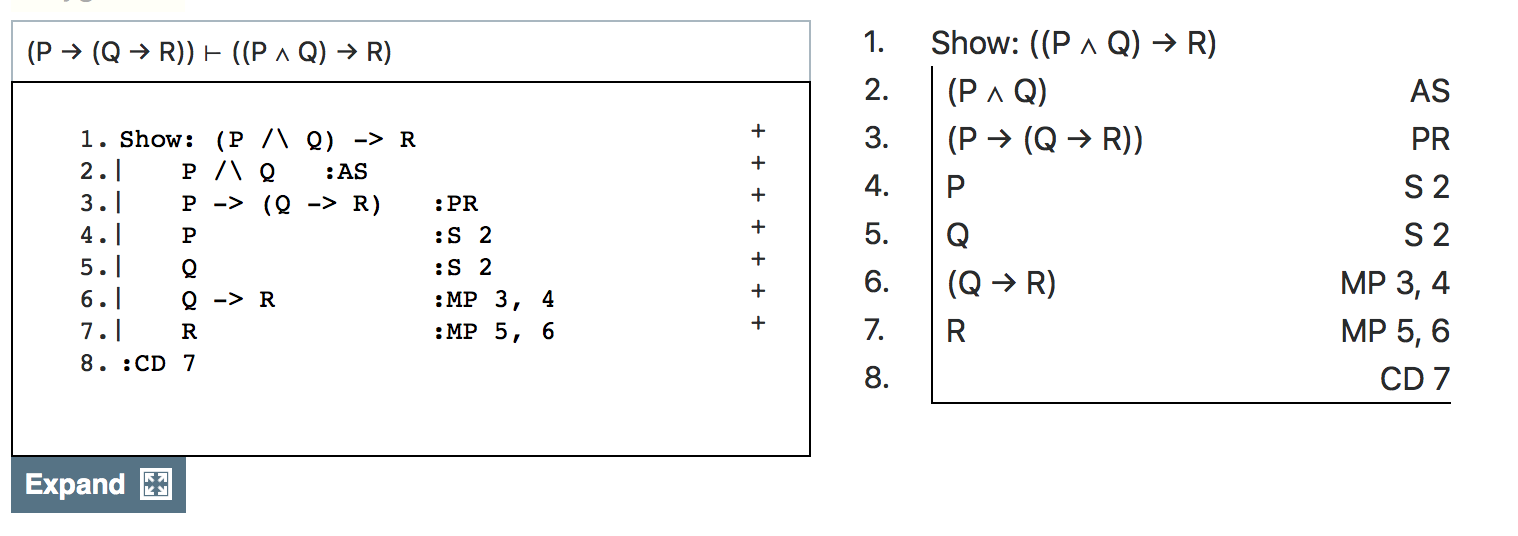
\includegraphics{../images/class05/Class-05-4.png}
\caption{\(P \rightarrow (Q \rightarrow R) \vdash (P \wedge Q) \rightarrow R\)}
\end{figure}

\end{frame}

\begin{frame}[fragile]{Text Version of Proof}
\protect\hypertarget{text-version-of-proof}{}

\begin{verbatim}
1. Show: (P /\ Q) -> R
2.    P /\ Q   :AS
3.    P -> (Q -> R)   :PR
4.    P               :S 2
5.    Q               :S 2
6.    Q -> R          :MP 3, 4
7.    R               :MP 5, 6
8. :CD 7
\end{verbatim}

\end{frame}

\begin{frame}{Reverse Direction}
\protect\hypertarget{reverse-direction}{}

\begin{figure}
\centering
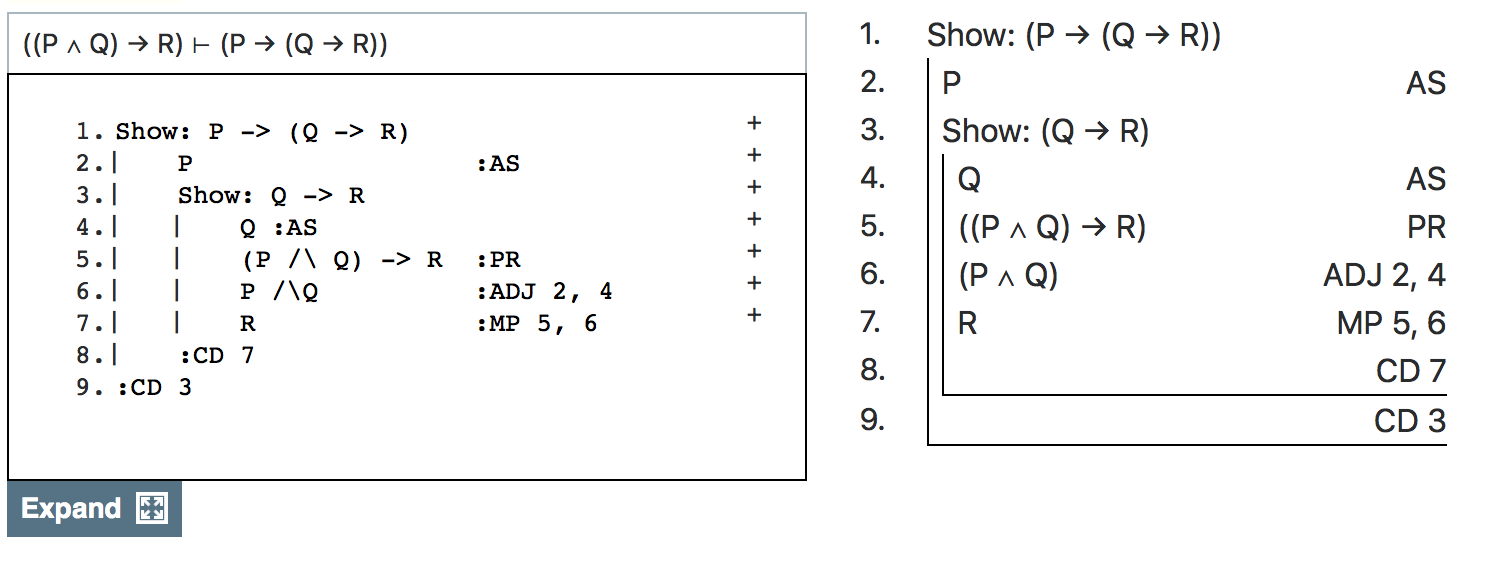
\includegraphics{../images/class05/Class-05-3.png}
\caption{\((P \wedge Q) \rightarrow R \vdash P \rightarrow (Q \rightarrow R)\)}
\end{figure}

\end{frame}

\begin{frame}[fragile]{Text Version of Proof}
\protect\hypertarget{text-version-of-proof-1}{}

\begin{verbatim}
1. Show: P -> (Q -> R)
2.     P                  :AS
3.     Show: Q -> R
4.         Q :AS
5.         (P /\ Q) -> R  :PR
6.         P /\Q          :ADJ 2, 4
7.         R              :MP 5, 6
8.     :CD 7
9. :CD 3
\end{verbatim}

\end{frame}

\begin{frame}{For Next Time}
\protect\hypertarget{for-next-time}{}

We'll talk about the rules for disjunction.

\end{frame}

\end{document}
